%%%%%%%%%%%%%%%%%%%%%%%%%%%%%%%%%%%%%%%%%%%%%%%%%%%%%%%%%%%%%%%%%%%%%%%%%%%
%%%%%%%%		 Proyecto Fin de Carrera		   %%%%%%%%
%%%%%%%%	       Presentación de diapositivas		   %%%%%%%%
%%%%%%%%%%%%%%%%%%%%%%%%%%%%%%%%%%%%%%%%%%%%%%%%%%%%%%%%%%%%%%%%%%%%%%%%%%%

\documentclass[utf8, compress]			{beamer}

%%%%%%%%%%%%%%%%%%%%%%%%%        Preámbulo        %%%%%%%%%%%%%%%%%%%%%%%%%

%---------------------------------beamer----------------------------------%

\mode<presentation>
{
    \useinnertheme{rounded}
    \useoutertheme[subsection=true]{miniframes}
    \useoutertheme{split}
    \useoutertheme{shadow}
    \setbeamertemplate{headline}[miniframes theme]{}
    \defbeamertemplate{footline}{pfc slides footline}{
	\leavevmode %
	\hbox{\begin{beamercolorbox} %
	    [wd		= .58\paperwidth, %
	     ht		= 2.5ex, %
	     dp		= 1.125ex, %
	     leftskip	= .3cm plus1fill, %
	     rightskip	= .3cm]{author in head/foot} %
	    \usebeamerfont{author in head/foot}\insertshorttitle
	  \end{beamercolorbox} %
	  \begin{beamercolorbox} %
	    [wd		= .38\paperwidth, %
	     ht		= 2.5ex, %
	     dp		= 1.125ex, %
	     leftskip	= .3cm, %
	     rightskip	= .3cm plus1fil]{title in head/foot} %
	    \usebeamerfont{title in head/foot}\insertshortinstitute
	  \end{beamercolorbox}} %
    	\vskip0pt %
    }
    \setbeamertemplate{footline}[pfc slides footline]{}
    \setbeamertemplate{frametitle}[shadow theme]{}
    \setbeamertemplate{itemize items}[circle]{}
    \setbeamertemplate{enumerate items}[circle]{}
    \setbeamertemplate{sections/subsections in toc}[circle]{}
    \setbeamertemplate{title page}{
	\vbox{}
	\vfill
	\begin{center}
	    \begin{beamercolorbox}[sep=8pt,center]{institute}
		\usebeamerfont{author}\insertinstitute
	    \end{beamercolorbox}
	    \inserttitlegraphic
	    \vskip.4em\par
	    \begin{beamercolorbox}[sep=8pt,center,rounded=true]{title}
		\usebeamerfont{title}\inserttitle
	    \end{beamercolorbox}
	    \vskip.4em\par
	    \begin{beamercolorbox}[sep=8pt,center]{date}
		\usebeamerfont{date}\insertdate
	    \end{beamercolorbox}
	    \begin{beamercolorbox}[sep=8pt,right]{author}
		\usebeamerfont{institute}\insertauthor
	    \end{beamercolorbox}
	\end{center}
	\vfill
    }
    \usecolortheme{orchid}
    \usecolortheme{whale}
}

%--------------------------------\beamer----------------------------------%

\usepackage[spanish]					{babel}
\usepackage[T1]						{fontenc}
\usepackage[altbullet, nofontinfo]			{lucidabr}
\usepackage						{graphicx}
\usepackage{array, booktabs, listings, multimedia}


%--------------------------------listings---------------------------------%
\lstloadlanguages{Matlab}

\lstset{language      = Matlab,
	basicstyle    = \ttfamily,
	keywordstyle  = \sffamily\bfseries,
	extendedchars = true,
	breaklines,
	captionpos    = b,
	morekeywords  = {addchannel,     analoginput, catch,
	datadqcallback,	 daqfind,        daqhwinfo,   errordlg,
	gcbo,            getdata,        guidata,     localDaqCallback,
	peekdata,        single_channel, start,       stop,
	strcmpi,	 trigger,        try,         warning}
}

\lstdefinestyle{displayed}{
	float            = tpbh,           tabsize     = 5,
	abovecaptionskip = \bigskipamount, gobble      = 4,
	xleftmargin      = .082\textwidth, numbers     = left,
	numberstyle      = \tiny,          numbersep   = 5pt
}
%-------------------------------\listings---------------------------------%

\graphicspath{{./pictures/}{../pictures/}}			% graphics

\title[ENDUS: Sistema de medida y aplicación en palmeras in vivo.]{
    Desarrollo de sistema de medida por ultrasonidos de baja frecuencia. \\
    Aplicación al análisis de palmeras in vivo.
}

\newlength{\director}
\settowidth\director{\usebeamerfont{institute}DIRECTOR: Alberto Rodríguez
    Martínez}

\author[José Ramón Gisbert Valls]{
    \vbox{
	\makebox[\director][r]{AUTOR: José Ramón Gisbert Valls}
	\makebox[\director][r]{DIRECTOR: Alberto Rodríguez Martínez}
    }
}

\institute[Universidad Miguel Hernández de Elche]{
    Universidad Miguel Hernández de Elche \medskip\par
    Escuela Politécnica Superior de Elche
}

\date[Septiembre --- 2011]{
    Proyecto Fin de Carrera \\
    Septiembre --- 2011
}

\titlegraphic{
    
\includegraphics[viewport = 0 524 152 678, clip, height = 1.4cm,
	keepaspectratio]{logo.pdf}
}

\logo{
    
\includegraphics[viewport = 0 524 152 678, clip, height = .8cm,
	keepaspectratio]{logo.pdf}
}

% Convenios tipográficos: siglas (primera vez), siglas, funciones,
% argumentos, propiedades, atributos de propiedades, nombres de canal o
% puerto
\newcommand\psig[1]{\emph{\MakeTextUppercase{#1}}}
\newcommand\sig [1]{\textsc{\MakeTextLowercase{#1}}}
\newcommand\func[1]{\texttt{#1}}
\newcommand\argu[1]{\texttt{#1}}
\newcommand\prop[1]{\textsf{#1}}
\newcommand\atr [1]{\textsf{#1}}
\newcommand\can [1]{\sig{#1}}

% Palabras predefinidas
\newcommand\matlab{\sig{MATLAB}}
\newcommand\kpci  {\sig{KPCI}-3108}
\newcommand\datx  {\sig{DAT}}
\newcommand\gui   {\sig{GUI}}
\newcommand\guide {\sig{GUIDE}}
\newcommand\pc    {\sig{pc}}
\newcommand\ram   {\sig{ram}}
\newcommand\AOUA  {\ensuremath{\mu}\sig{a}741}
\newcommand\kms   {kmus/s}

%%%%%%%%%%%%%%%%%%%%%%%%         Contenido         %%%%%%%%%%%%%%%%%%%%%%%%

\begin{document}


\frame[plain]{\titlepage}

\begin{frame}{Índice}
    \tableofcontents
\end{frame}

\begin{frame}{Objetivos}
    \begin{enumerate}
	\item Desarrollo de un \alert{sistema de medida por ultrasonidos}
	    que proporcione información visual de la señal de forma
	    instantánea y que permita extraer una versión digitalizada de
	    la señal y de su espectro en frecuencias.
	\item Realización de un \alert{estudio preliminar} que determine la
	    existencia de una relación entre los parámetros medidos en un
	    ENDUS y las condiciones a las que se encuentra expuesta una
	    palmera.
    \end{enumerate}
\end{frame}


\section{Desarrollo del sistema de medida}

\subsection{Subsistema físico}

\begin{frame}{Transductores y requisitos de acondicionamiento}
    \begin{itemize}
	\item Son transductores activos piezoeléctricos.
	\item Requisitos de acondicionamiento del actuador:
	    \begin{itemize}
		\item Máxima transferencia de potencia.
		\item Máxima potencia transmitida.
		\item Señal pulsada.
		\item Frecuencia de oscilación de 40 kHz.
	    \end{itemize}
	\item Requisitos de acondicionamiento del sensor:
	    \begin{itemize}
		\item Adaptación de impedancias.
		\item Ganancia elevada.
		\item Ancho de banda suficiente para acomodar la señal.
		\item Supresión de la componente en modo común.
	    \end{itemize}
    \end{itemize}
\end{frame}


\subsection{Subsistema de adquisición}

\begin{frame}{Tarjeta de adquisición digital}
    \alert{figura}
\end{frame}

\begin{frame}{Características de la tarjeta}
    \begin{itemize}
	\item Interfaz PCI (velocidad máxima de transferencia 132 MB/s).
	\item Subsistema de adquisición de señales analógicas.
	\item Subsistema generador de señales analógicas (2 canales de
	    salida analógica).
	\item Subsistema de entrada/salida digital (4 registros de 8~bits
	    de propósito general).
    \end{itemize}
\end{frame}

\begin{frame}{Características del subsistema de adquisición}
    \begin{itemize}
	\item Rendimiento máximo de muestreo de 100 kmus/s.
	\item 16 canales de entrada analógica configurables por software.
	\item Amplificador de instrumentación implementado internamente en
	    la tarjeta, ganancia configurable por software.
	\item Conversor A/D de 16 bits de precisión.
	\item Cola de muestreo de 256 posiciones.
	\item Buffer FIFO con capacidad para 2048 muestras.
    \end{itemize}
\end{frame}

\begin{frame}{Caja de conexiones}
    \begin{itemize}
	\item Necesidad de una interfaz para la realización de las pruebas.
	\item Diseño y construcción de una caja de conexiones:
	    \begin{itemize}
		\item Cables terminados en conectores macho mini-D.
		\item Identificación de los puertos de entrada/salida.
		\item Localización del cable correspondiente a cada puerto.
		\item Realización de un mapa de colores.
		\item Construcción de la caja.
	    \end{itemize}
    \end{itemize}
\end{frame}

\newlength{\exterior}
\settoheight\exterior{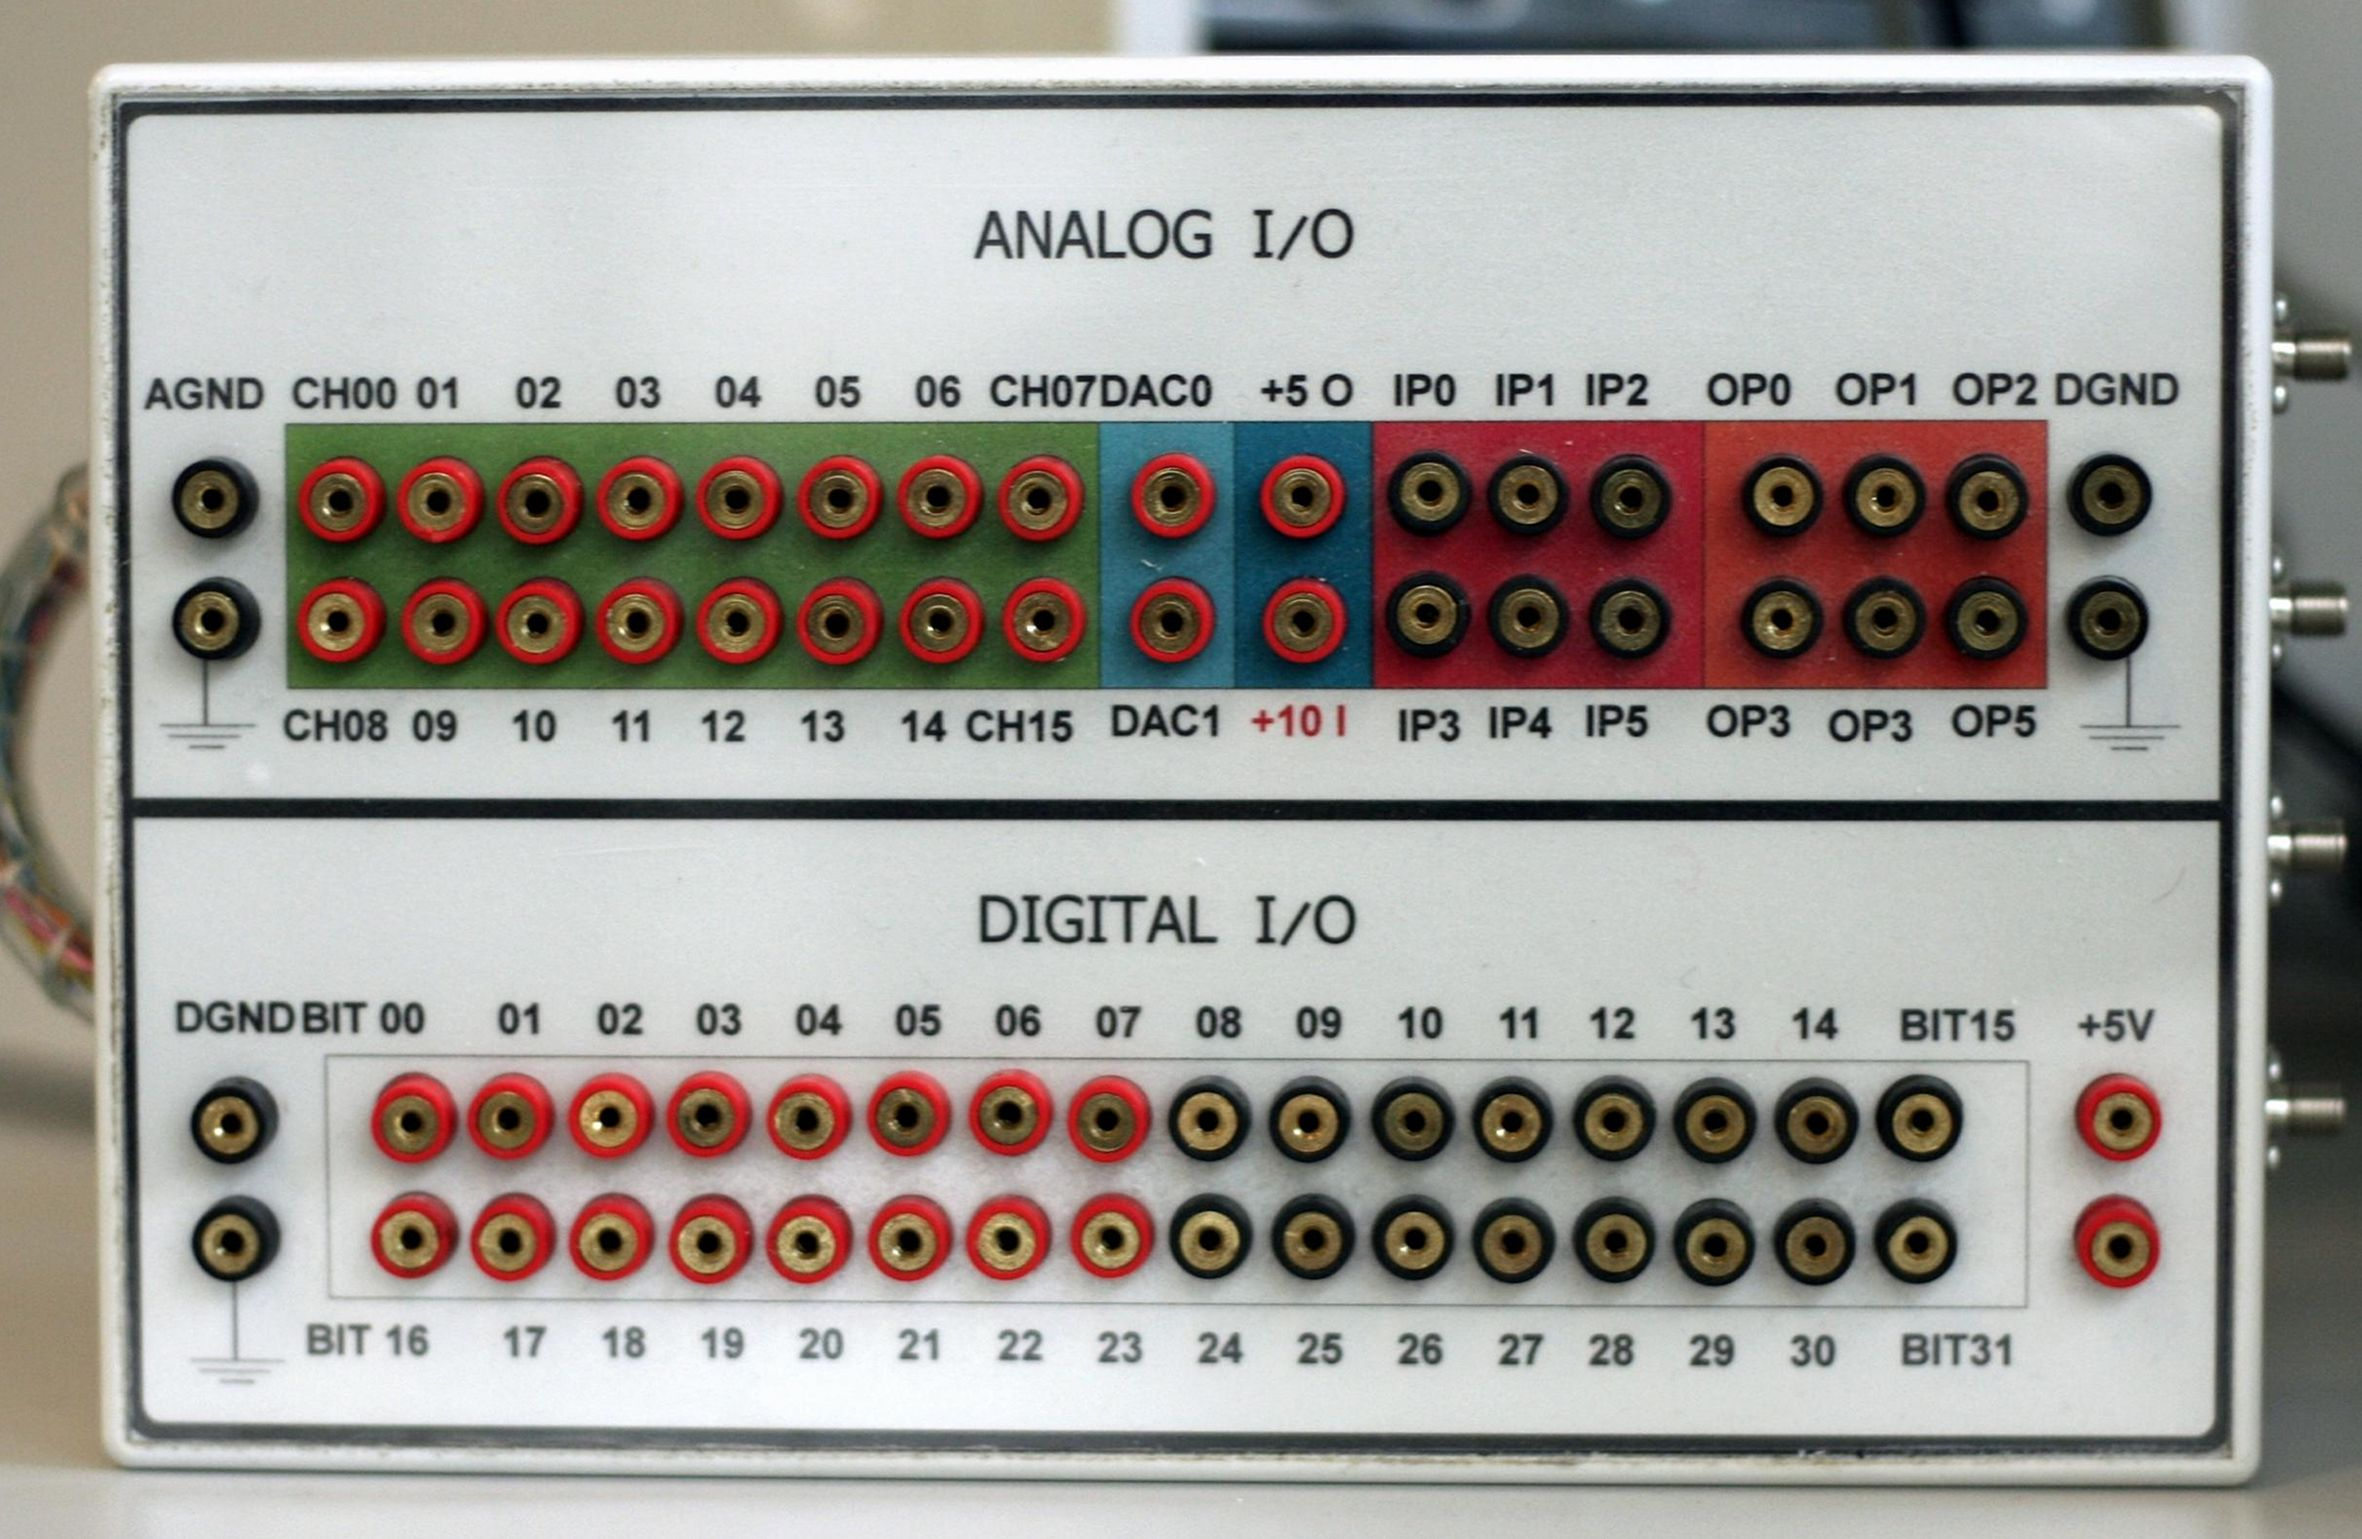
\includegraphics[angle=90]{exterior.jpg}}
\newlength{\interior}
\settowidth\interior{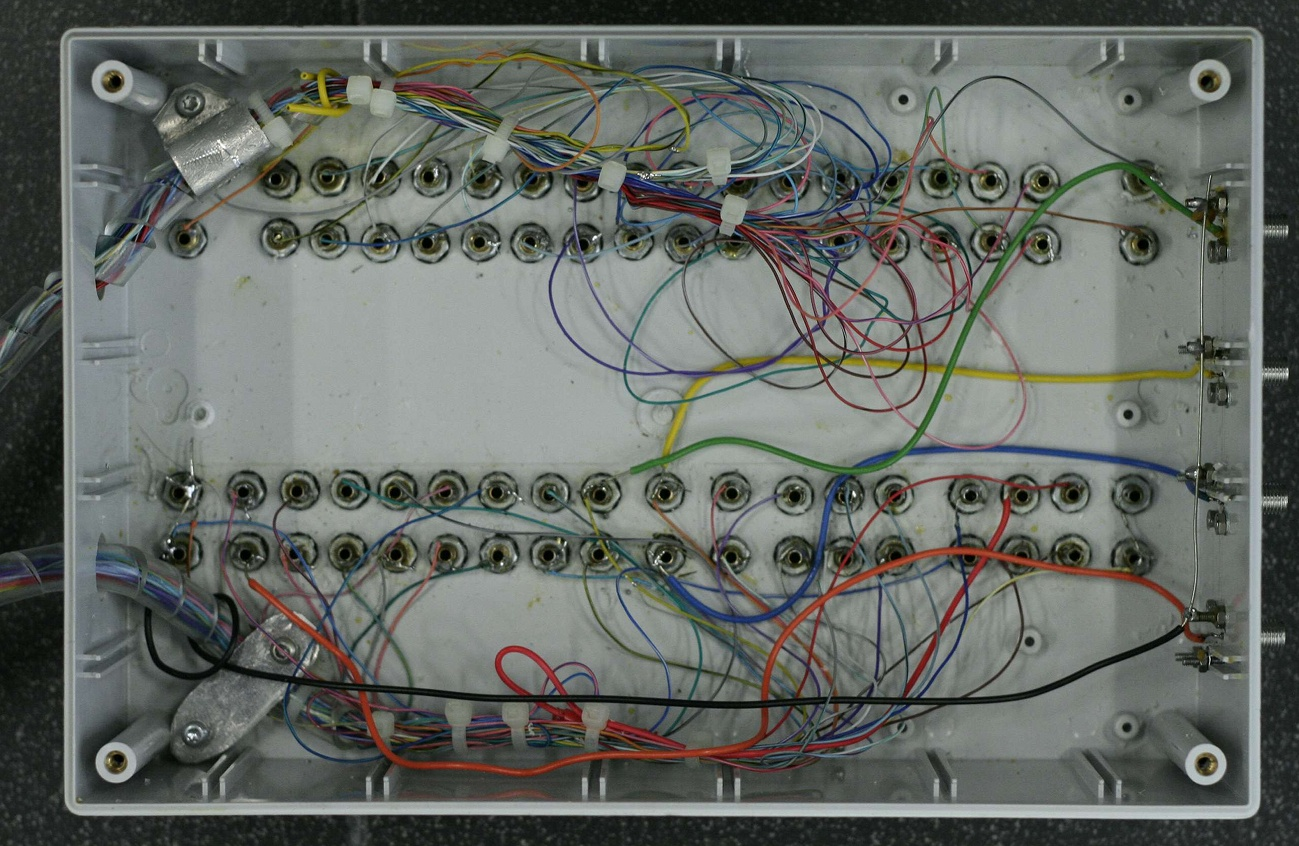
\includegraphics[angle=90]{interior.jpg}}

\begin{frame}{Caja de conexiones}
    \begin{figure}
	\hfill
	\begin{minipage}[top][\exterior][c]{\interior}
	    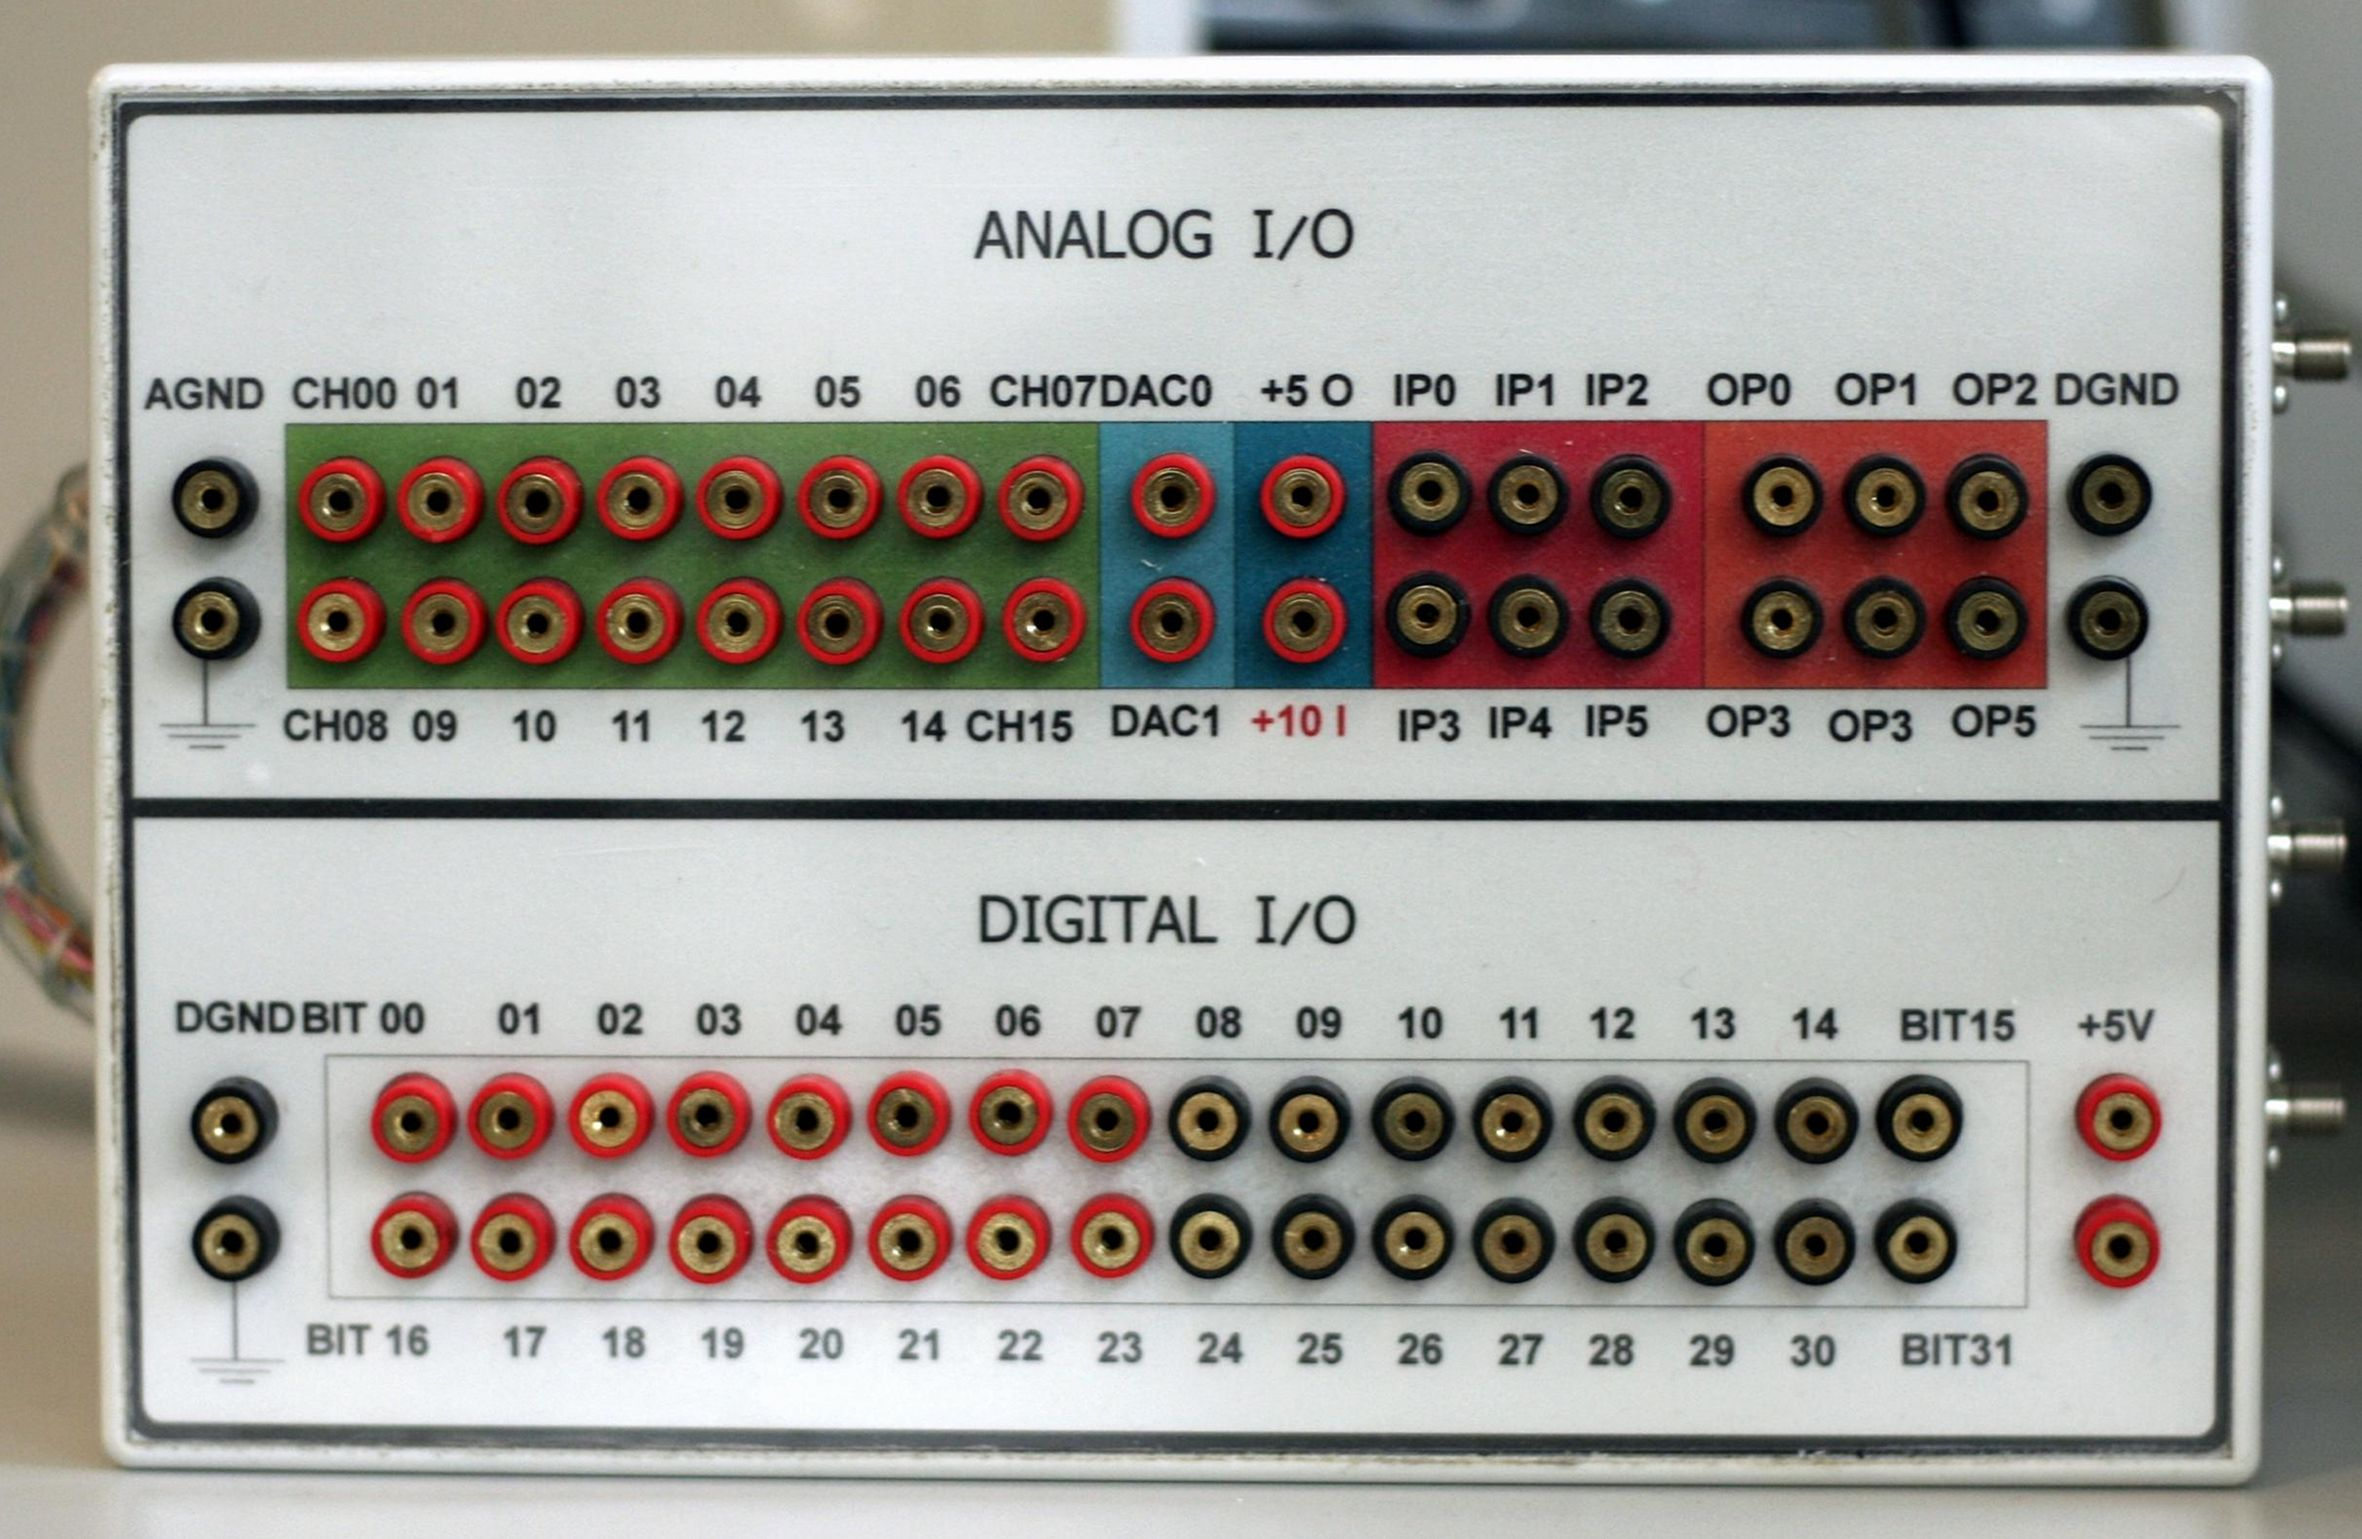
\includegraphics[angle=90]{exterior.jpg}
	\end{minipage}
	\hspace{1.5em}
	\begin{minipage}[top][\exterior][c]{\interior}
	    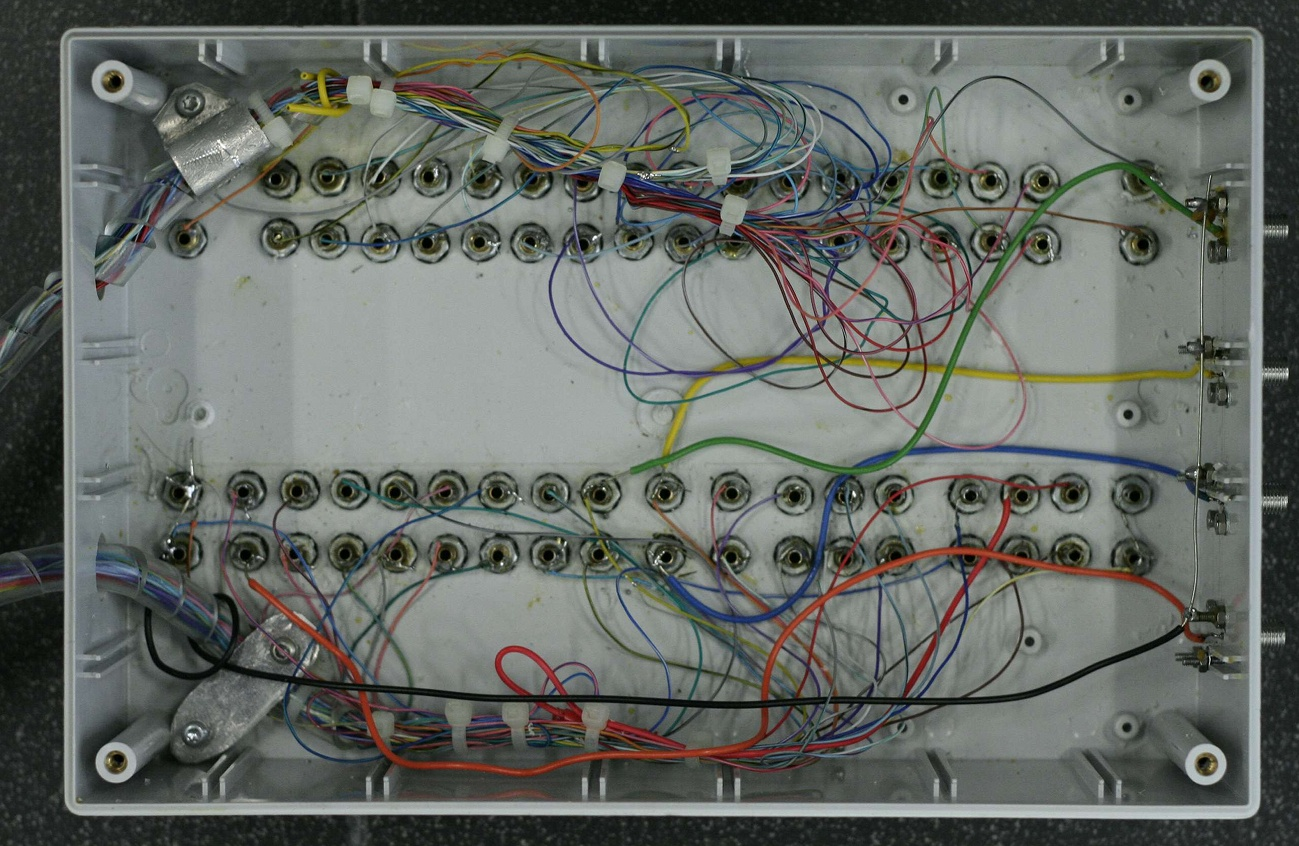
\includegraphics[angle=90]{interior.jpg}
	\end{minipage}
	\hfill
	\caption{Vistas interna y externa de la caja de conexiones.}
	\label{fig:connectionbox}
    \end{figure}
\end{frame}


\subsection{Subsistema de control y presentación}

\begin{frame}{Objetivos de programación}
    \begin{itemize}
	\item Valor numérico instantáneo de la señal.
	\item Media aritmética de las muestras tomadas durante un
	    periodo de 250 ms.
	\item Representación gráfica de la señal.
	\item Representación gráfica del espectro instantáneo de la
	    señal.
    \end{itemize}
\end{frame}

\begin{frame}[fragile]{Proceso de aprendizaje para la utilización del SDK}
    \begin{itemize}
	\item MATLAB (MATrix LABoratory), kit de desarrollo de software.
	\item GUIDE (Graphical User Interface Development Environment),
	    desarrollo de interfaces gráficas.
	\item DAT (Data Acquisition Toolbox), manejo de dispositivos de
	    adquisición y generación de señales.
	    \vspace{\baselineskip}
	    \begin{lstlisting}
		handles.ai = analoginput(`keithley');
		guidata(hObject, handles);
	    \end{lstlisting}
    \end{itemize}
\end{frame}

\begin{frame}{Diseño conceptual}
    \begin{figure}
	\hfill
	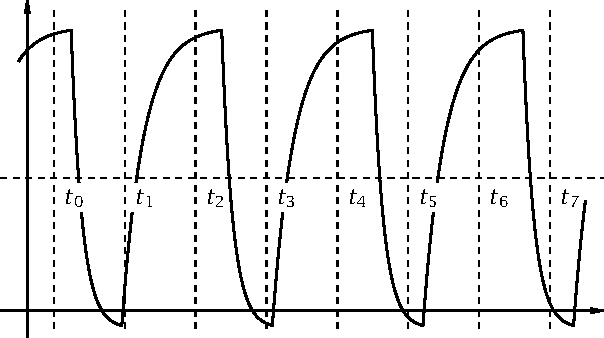
\includegraphics[height=25mm, keepaspectratio]{ventanas.pdf}
	\hspace{1em}
	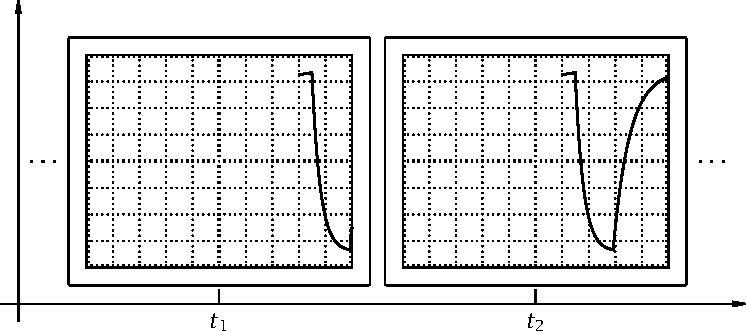
\includegraphics[height=25mm, keepaspectratio]{continuo.pdf}
	\hfill
	\caption{Modo de representación continuo.}
	\label{fig:continuous}
    \end{figure}
\end{frame}

\begin{frame}{Diseño conceptual}
    \begin{figure}
	\hfill
	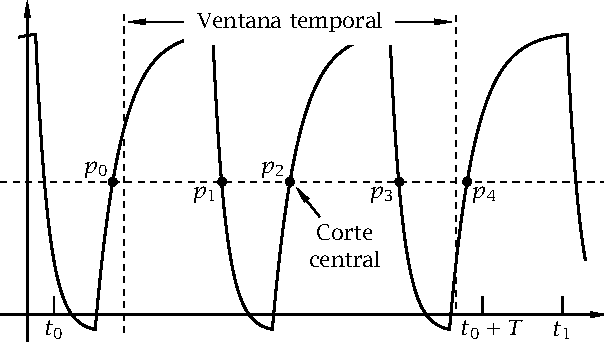
\includegraphics[height=25mm, keepaspectratio]{ventana.pdf}
	\hspace{3em}
	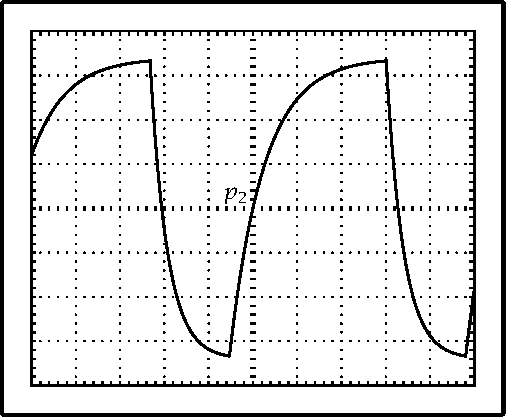
\includegraphics[height=25mm, keepaspectratio]{disparo.pdf}
	\hfill
	\caption{Modo de representación disparado.}
	\label{fig:triggered}
    \end{figure}
\end{frame}


\section{Estudio preliminar de la madera de palmera}

\subsection{Teoría de los ENDUS}

\begin{frame}{Características de los ultrasonidos}
    \begin{itemize}
	\item Son perturbaciones mecánicas que viajan a través de un medio
	    elástico.
	\item Banda de frecuencia de 20 kHz a 1000 MHz (límite
	    tecnológico).
	\item Banda de frecuencia utilizada en ENDUS de 20 kHz a 25~MHz.
	\item Sus propiedades son invariantes con la frecuencia.
	\item Cuatro tipos de onda ultrasónica: longitudinales,
	    transversales, de superficie y ondas de Lamb.
    \end{itemize}
\end{frame}

% Particularidades de los ENDUS
\begin{frame}{Ensayos no destructivos por ultrasonidos}
    \begin{itemize}
	\item Campo generado por un transductor cilíndrico, resolución de
	    un ensayo.
	\item Técnicas de transmisión y de pulso"=eco.
	\item Dispersión y ruido estructural o de grano.
	\item Técnicas de postprocesado destinadas a eliminar el ruido
	    estructural.
    \end{itemize}
\end{frame}


\subsection{Realización del estudio}

\begin{frame}{Objetivos del estudio}
    \begin{itemize}
	\item Interés en determinar las características del material.
	\item Pocas referencias que documenten la realización de ENDUS en
	    madera.
	\item Peculiaridades de la madera de palmera.
	\item Disponibilidad de unos transductores de impacto
	\item \alert{Sentar unas bases para la realización de estudios
	    posteriores.}
    \end{itemize}
\end{frame}

\begin{frame}{Peculiaridad de la madera de palmera}
    \alert{figura}
\end{frame}

\newlength{\heighteuca}
\settoheight\heighteuca{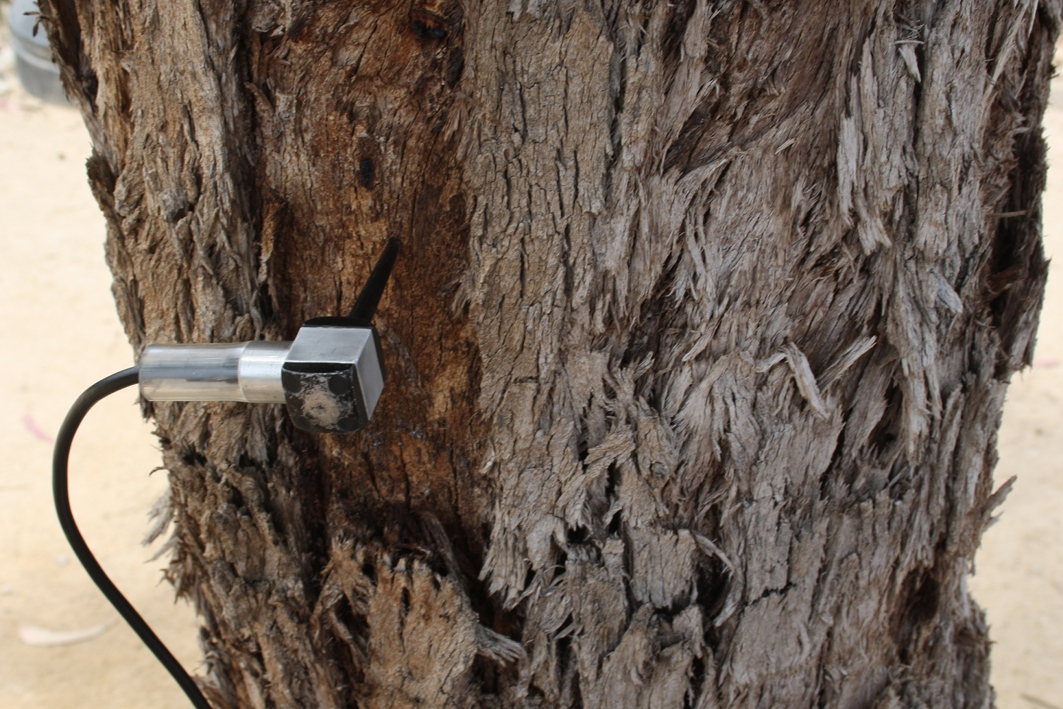
\includegraphics{meucalipto.jpg}}
\newlength{\widtheuca}
\settowidth\widtheuca{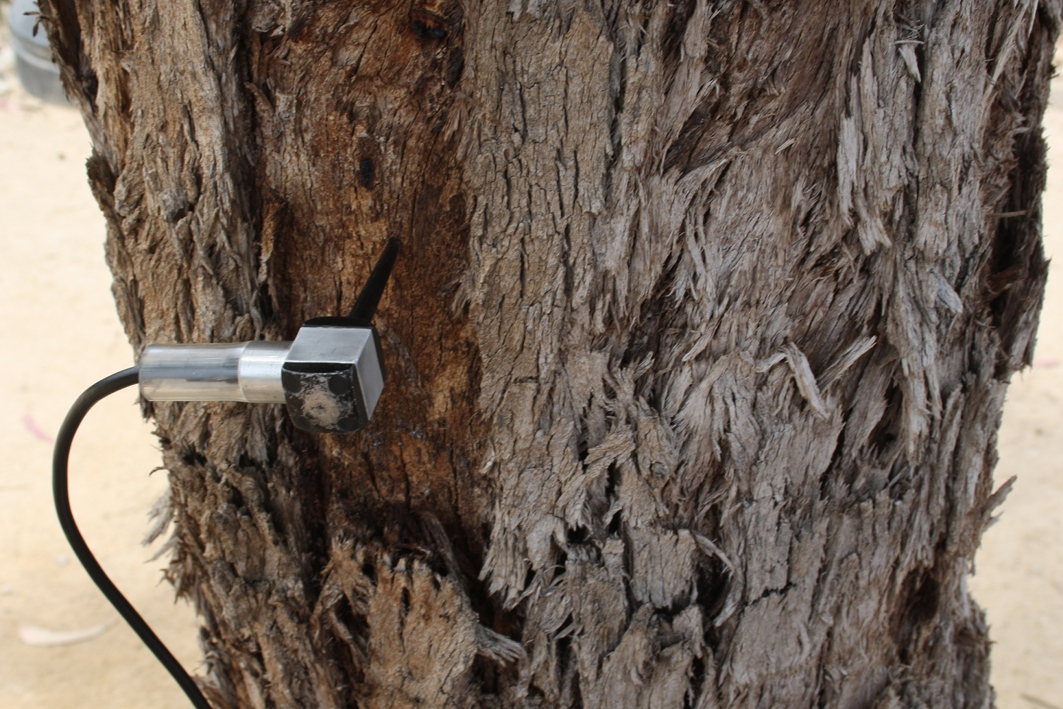
\includegraphics{meucalipto.jpg}}
\newlength{\widthpalm}
\settowidth\widthpalm{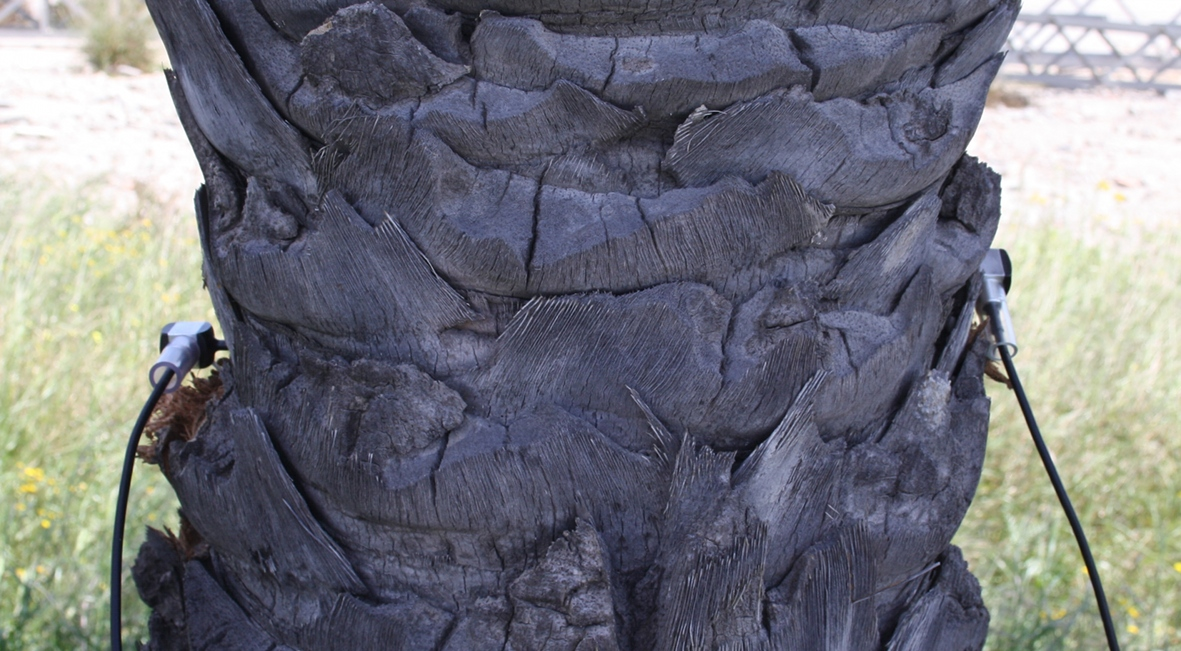
\includegraphics{mpalmera.jpg}}

\begin{frame}{Metodología}
    \alert{figura} 
\end{frame}

\begin{frame}{Metodología}
    \begin{figure}
	\begin{minipage}[top][\heighteuca][c]{\widthpalm}
	    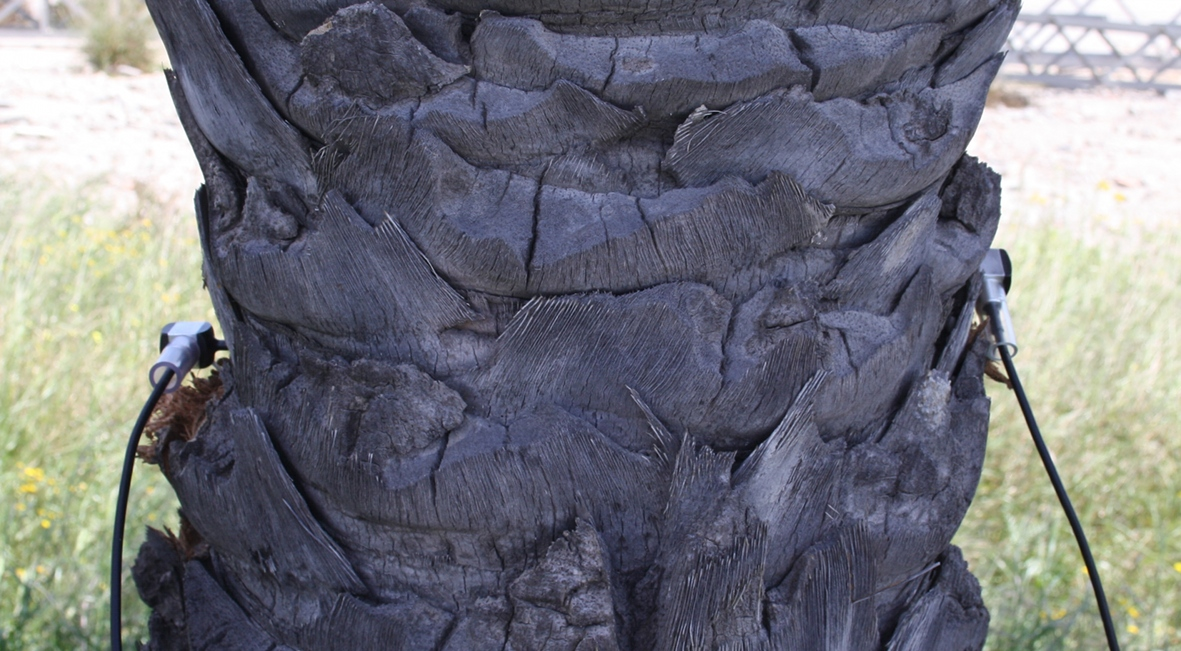
\includegraphics{mpalmera.jpg}
	\end{minipage}
	\hspace{.1em}
	\begin{minipage}[top][\heighteuca][c]{\widtheuca}
	    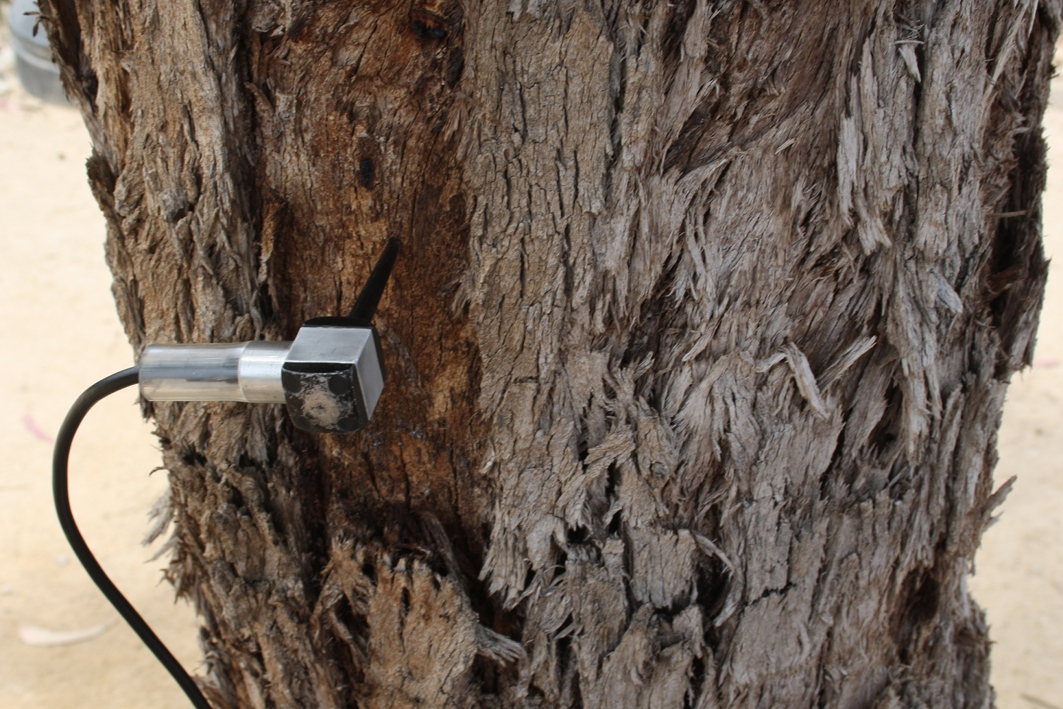
\includegraphics{meucalipto.jpg}
	\end{minipage}
	\caption{Medidas tomadas en una palmera y un eucalipto.}
	\label{fig:measures}
    \end{figure}
\end{frame}


\section[Resultados y conclusiones]{Resultados, conclusiones y futuras
    líneas de trabajo}

\subsection{Desarrollo del sistema de medida}

\begin{frame}{Prestaciones del sistema}
    \begin{center}
	\movie[showcontrols=true, height=60mm, width=106.67mm]
	    {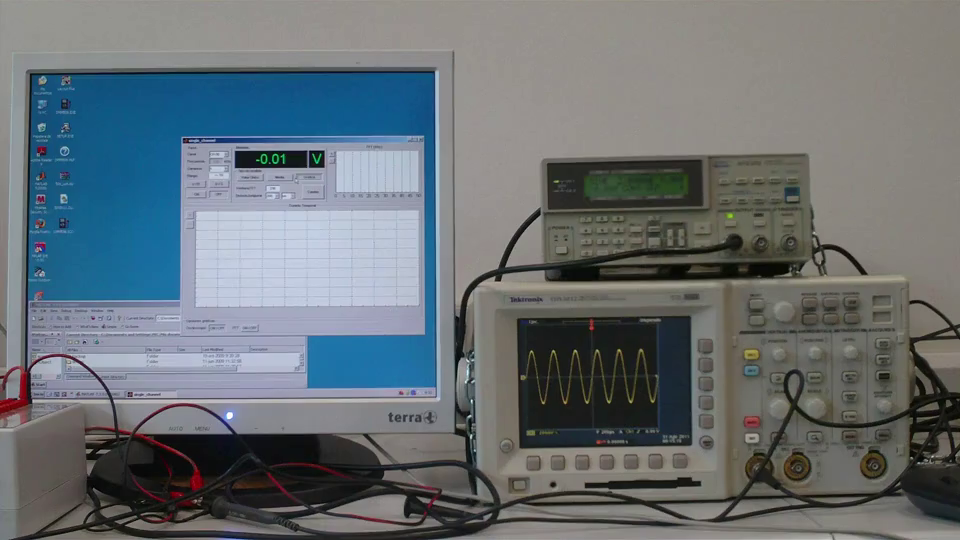
\includegraphics[height=60mm, width=106.67mm]{proyecto.png}}
	    {proyecto.mov}
    \end{center}
\end{frame}

\begin{frame}{Prestaciones del sistema}
    \begin{figure}
	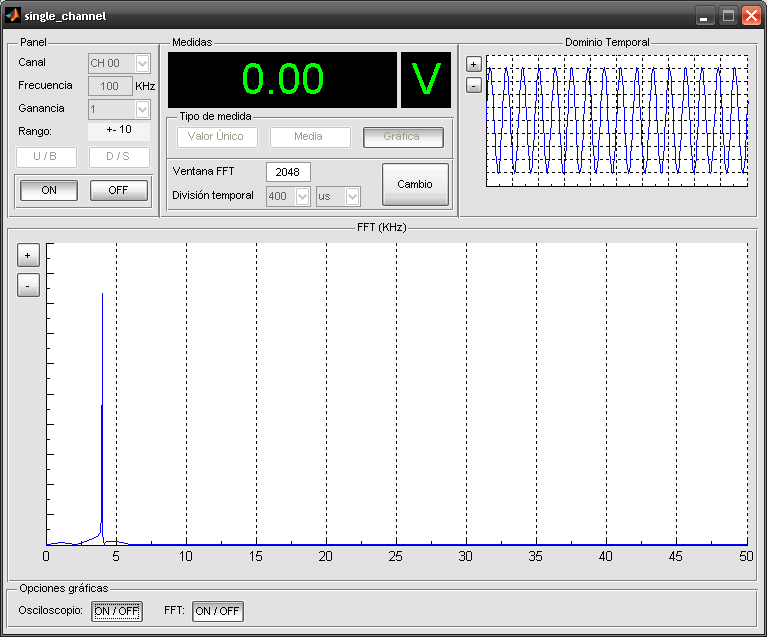
\includegraphics{softwarebis.png}
	\caption{Función del botón cambio.}
	\label{fig:softwarebis}
    \end{figure}
\end{frame}


\subsection{Estudio preliminar de la madera de palmera}

\begin{frame}{Resultados de los ensayos}
    \begin{figure}
	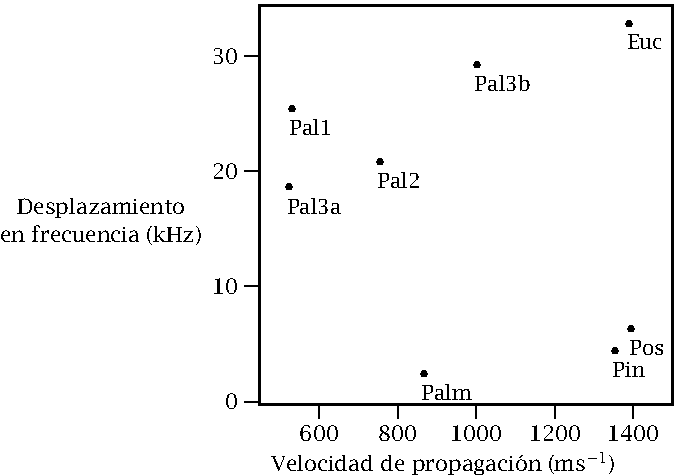
\includegraphics[height=55mm, keepaspectratio]{resultados.pdf}
	\caption{Resultados obtenidos en las pruebas}
	\label{fig:results}
    \end{figure}
\end{frame}


\subsection{Conclusiones y futuras líneas de trabajo}

\begin{frame}{Sistema de medida}
    \begin{itemize}
	\item Conclusiones:
	    \begin{itemize}
		\item Se ha desarrollado con éxito el sistema de medida.
		\item Se han implementado todas las prestaciones
		    requeridas.
	    \end{itemize}
	    \vspace{1ex}
	\item Futuras líneas de trabajo:
	    \begin{itemize}
		\item Limitación del sistema en frecuencia.
		\item Limitación de los transductores en potencia.
	    \end{itemize}
    \end{itemize}
\end{frame}

\begin{frame}{Estudio preliminar}
    \begin{itemize}
	\item Conclusiones:
	    \begin{itemize}
		\item Se observa una relación entre los resultados y el
		    tipo de ejemplar.
		\item Se observa una relación entre los resultados y el
		    estado del ejemplar.
		\item Se observa una relación entre los resultados y la
		    altura a la que se realiza la medida.
	    \end{itemize}
	\item Futuras líneas de trabajo:
	    \begin{itemize}
		\item Se recomienda un profundo estudio teórico y la
		    realización de más ensayos para determinar que relación
		    existen entre los resultados de un ENDUS y el estado
		    del ejemplar.
	    \end{itemize}
    \end{itemize}
\end{frame}


\end{document}
